\chapter{Drone Hardware}
\label{ch:drone}

The drone used at the time of writing this thesis is a Snapdragon drone with a Pixhawk flight controller and a VOXL2 embedded processor.

\begin{figure}[h]
\centering
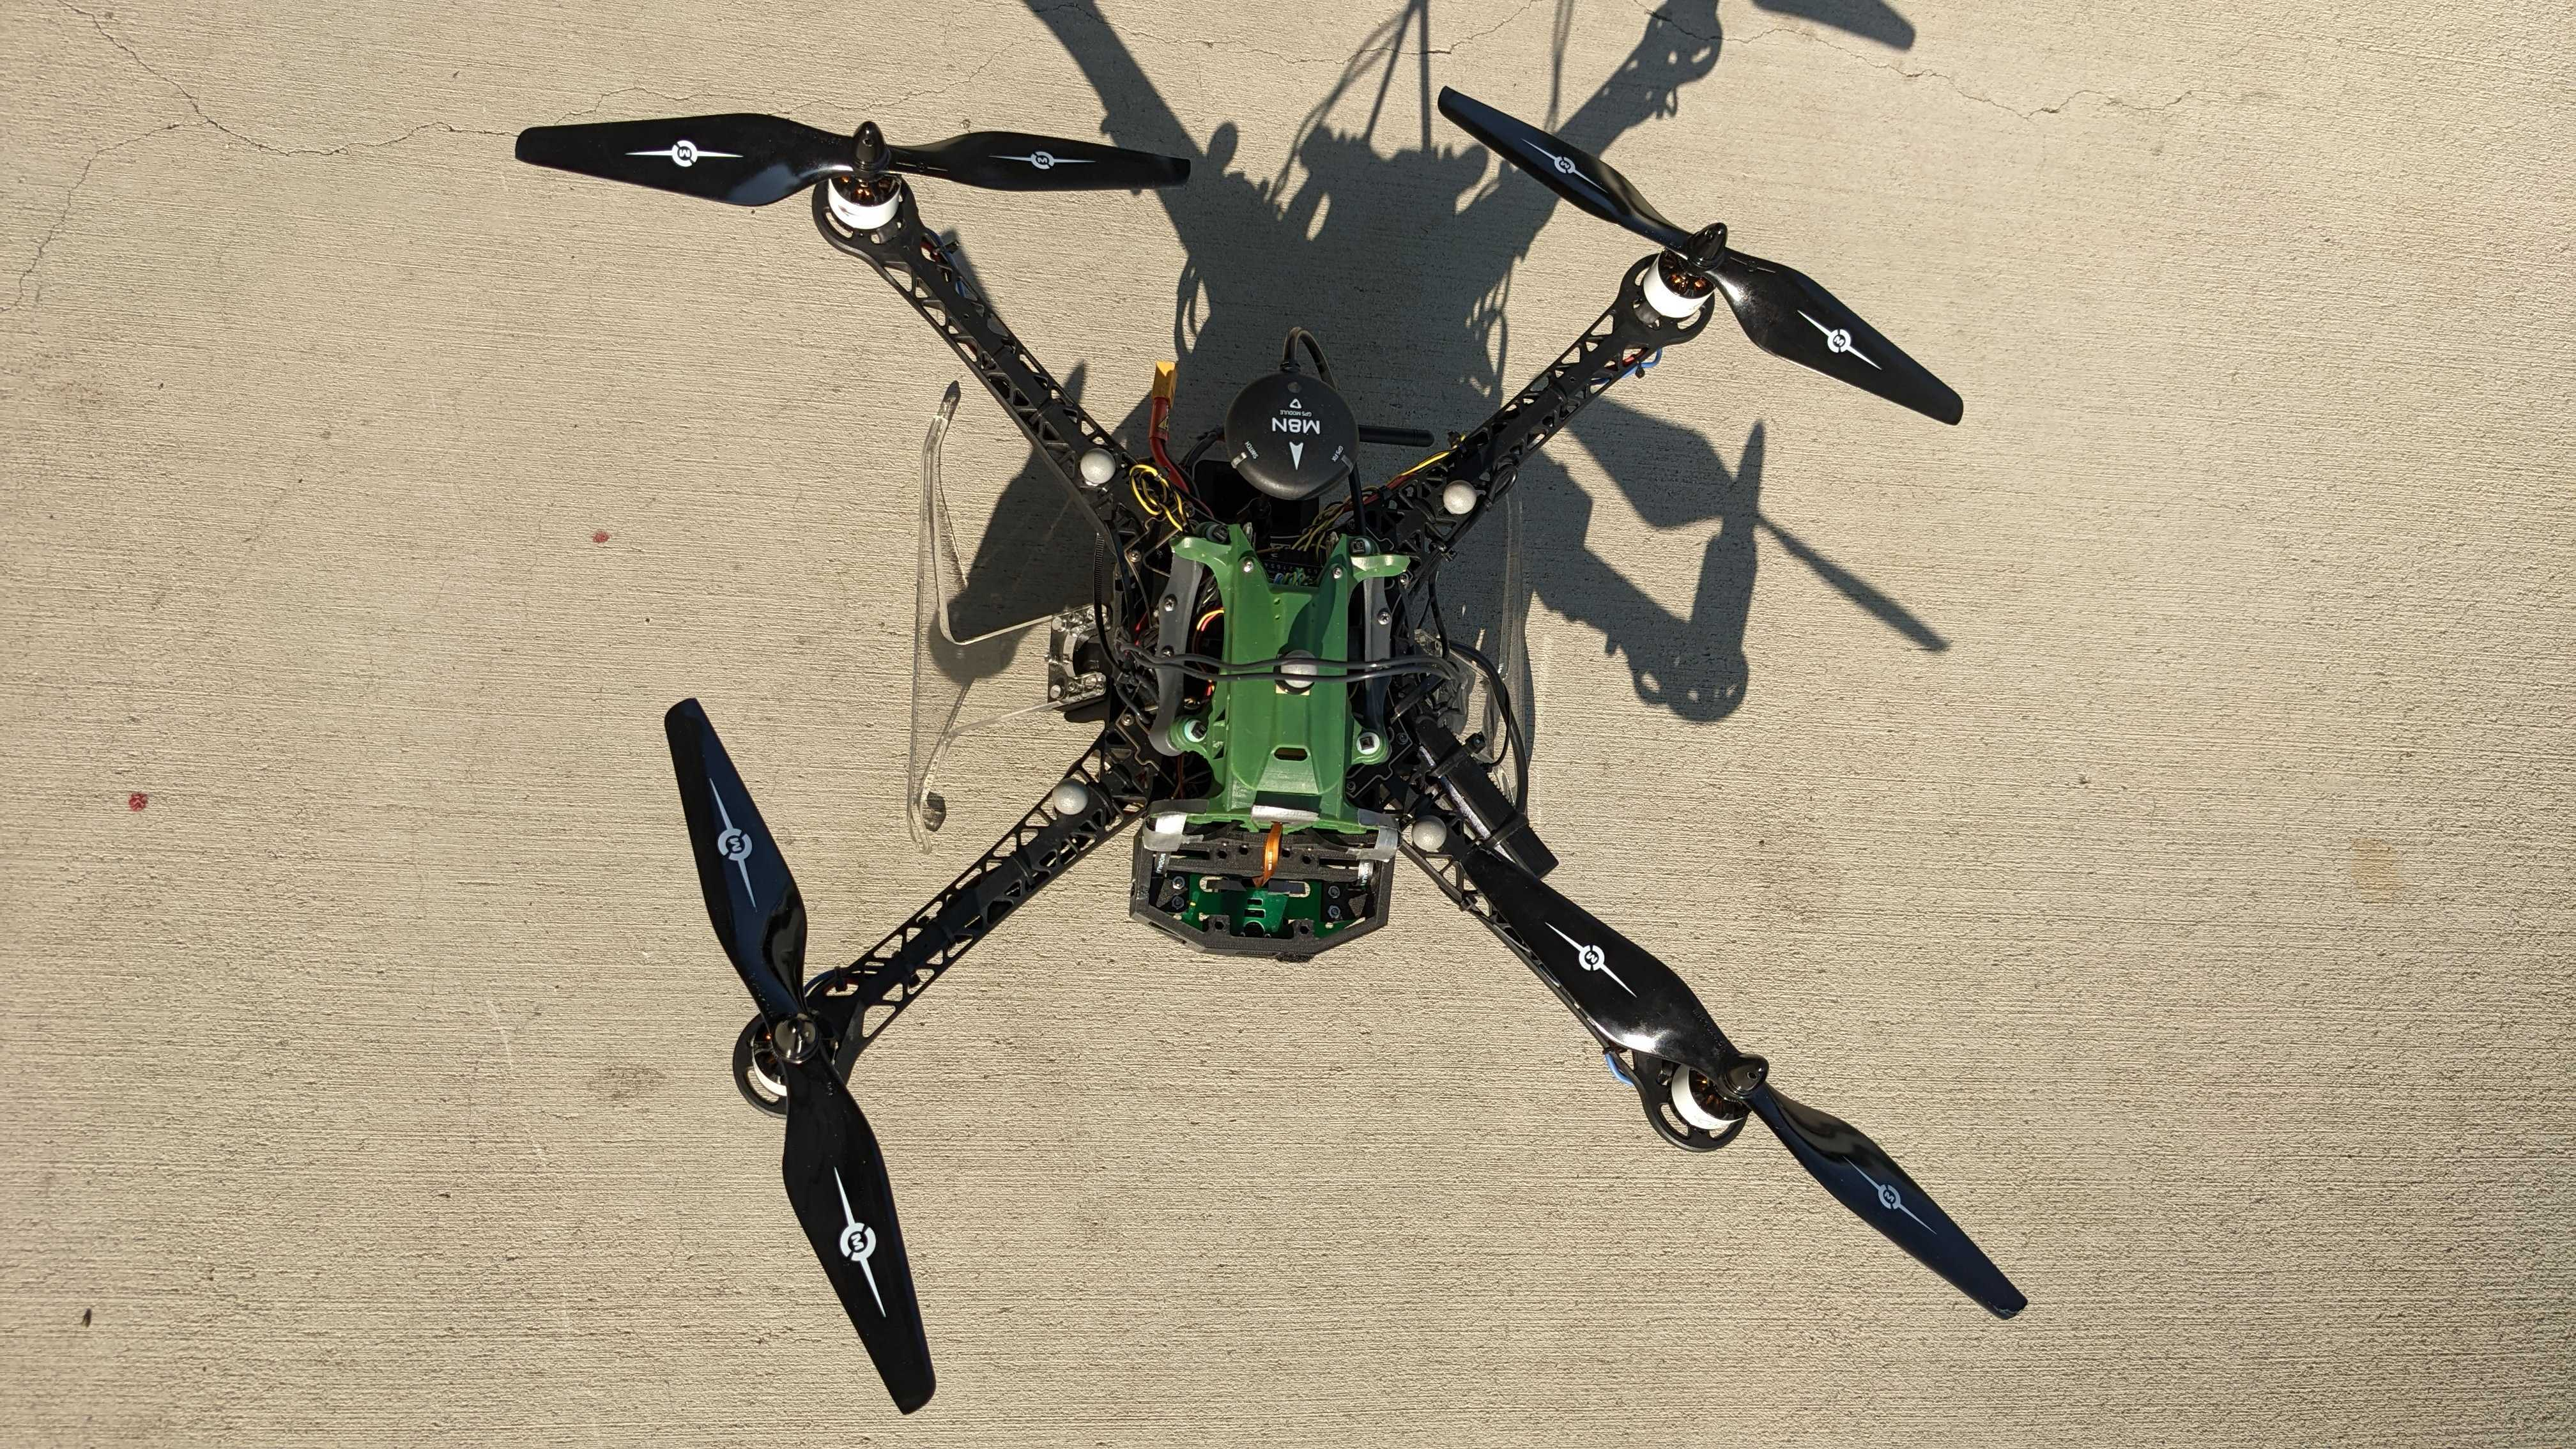
\includegraphics[scale=0.5]{images/appendix/Drone/drone.jpg}
\caption{Snapdragon drone setup}
\label{fig:appendix_drone_hardware}
\end{figure}

\cref{fig:appendix_drone_hardware} shows an image of the rotorcraft hardware used by LORNA. On this drone setup there is a tracking camera and a stereo camera.

The stereo camera marginally used for tests in this work is shown in \cref{fig:appendix_stereo_camera_hardware}. Note that the landing supports of the drone are significantly farther apart than for the model in the simulation. This is why the simulated stereo camera in Gazebo had to be placed further away from the drone while in reality it was mounted normally on the drone's body.

\begin{figure}[h]
    \centering
    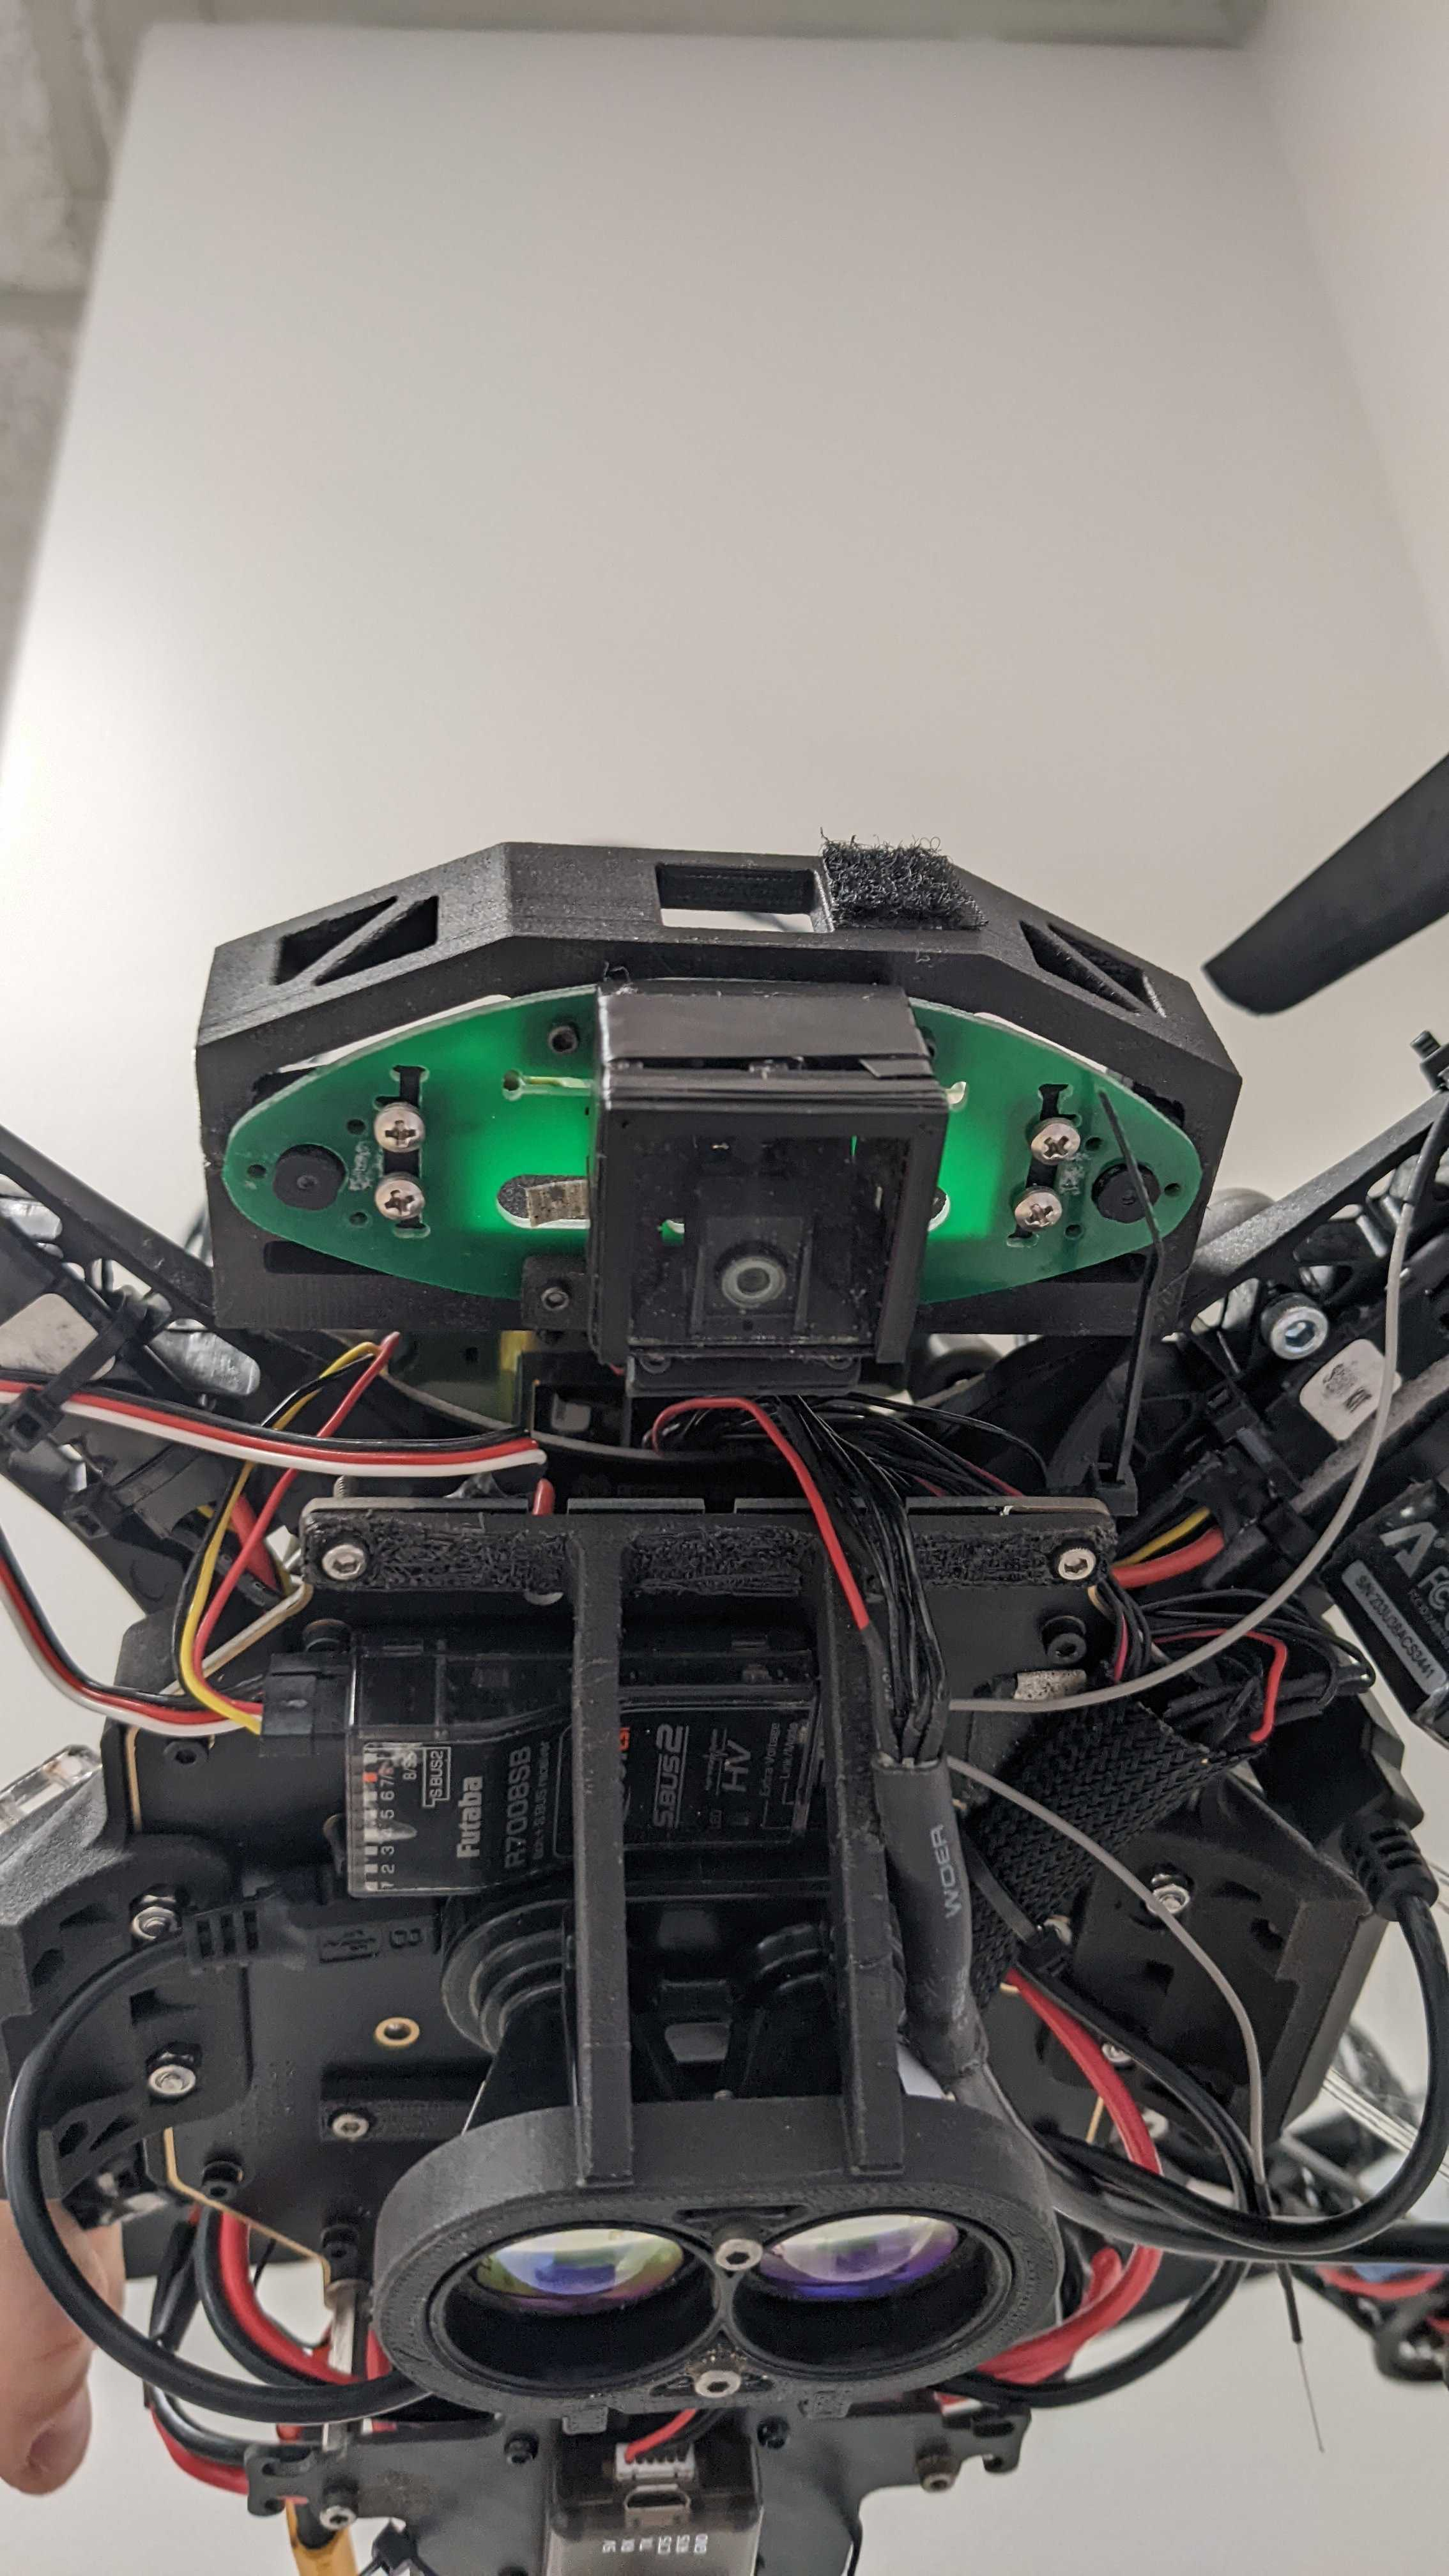
\includegraphics[scale=0.5]{images/appendix/Drone/stereo_cam.jpg}
    \caption{Stereo camera on physical drone}
    \label{fig:appendix_stereo_camera_hardware}
    \end{figure}